\IfFileExists{solve_stats/language_stats.pdf}{%
  \begin{frame}[c]{Language stats}
    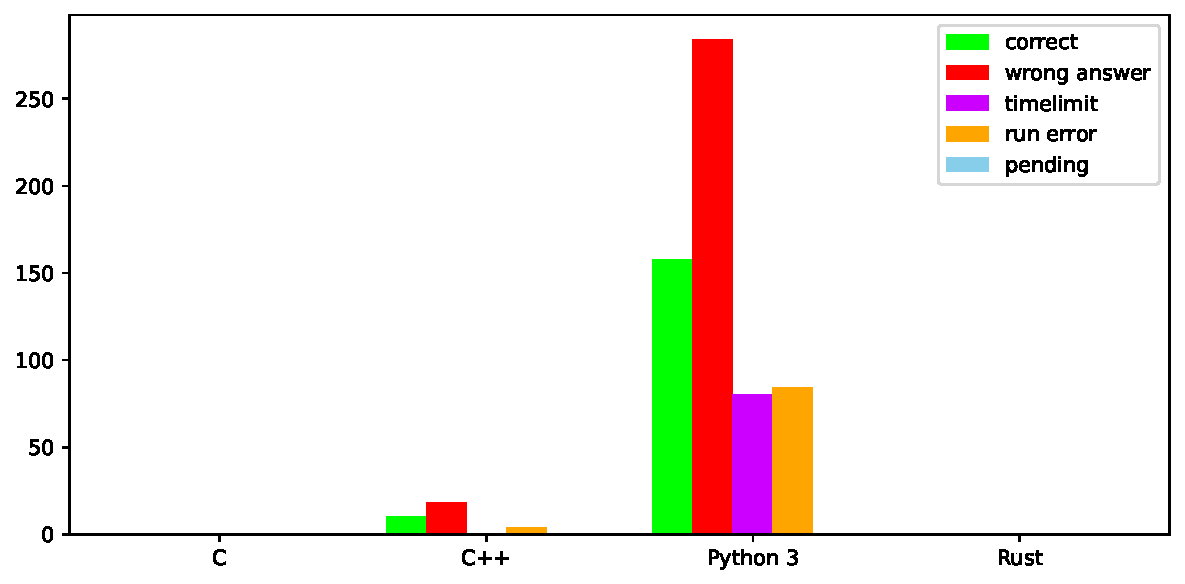
\includegraphics[width=\textwidth]{solve_stats/language_stats}%
  \end{frame}
}

\begin{frame}{Random facts}
    \begin{block}{Jury work}
      \begin{itemize}[<+->]
        % git rev-list --all -- main | wc -l
        \item 632 commits
        % bt stats
        %\item 681 secret test cases (last year: 486) ($\approx 57$ per problem!)
        %\item 248 jury solutions (last year: 232)
        % cd main ; for dir in */ ; do echo "$dir $(cloc --by-file ${dir}submissions/accepted | tail -n 4 | head -n 1)" ; done
        % cd main; for dir in */ ; do cloc --by-file ${dir}submissions/accepted | tail -n 4 | head -n 1 | tr -s ' ' | cut -d ' ' -f 4 ; done
        %\item The minimum\footnotemark{} number of lines the jury needed to solve all problems is
        %\[ 10 + 114 + 27 + 5 + 64 + 51 + 42 + 32 + 43 + 23 + 10 + 6 = 427 \]
        %On average $35.5$ lines per problem, up from $9.6$ in the BAPC
      \end{itemize}
    \end{block}
    %\footnotetext{\emph{After} codegolfing}
\end{frame}
